\documentclass[a4paper]{article}


\usepackage[margin = .9 in]{geometry}
\usepackage{graphicx}
\usepackage{xcolor}
\usepackage{setspace}
\usepackage[outline]{contour}
\usepackage[colorlinks=true,citecolor=blue , linkcolor = black]{hyperref}
\usepackage {fancybox}
\usepackage{amssymb}


\usepackage{amsmath, calc}

\usepackage{background}
\usepackage{lipsum}
\usetikzlibrary{calc}

\SetBgScale{1}
\SetBgAngle{0}
\SetBgColor{black}
\SetBgContents{
	
\begin{tikzpicture}[overlay,remember picture]
	\draw [line width=1pt,rounded corners=15pt,double]
	($ (current page.north west) + (1cm,-1cm) $)
	rectangle
	($ (current page.south east) + (-1cm,0.7cm) $);
	\end{tikzpicture}
}


\begin{document}
	
	\begin{titlepage}
	
		\definecolor{b1}{HTML}{010EFB}
		\definecolor{y1}{HTML}{FFFFFF}
	%   \pagecolor{y1}\afterpage{\nopagecolor}
		
		\centering
		\vspace*{2\baselineskip}
		\rule{\textwidth}{2pt}\vspace*{-\baselineskip}\vspace*{3pt}
		\rule{\textwidth}{0.4pt}
		\vspace{1pt}
		
		{\Huge \bf \emph{Statistics and Probabilities \\ In \\ Markov Chain}\\}
		\vspace{0.75\baselineskip}
		
		\rule{\textwidth}{0.4pt}\vspace*{-\baselineskip}\vspace{4pt}
		\rule{\textwidth}{2.5pt}\\
		
		\vspace{3\baselineskip}
		
		{\Large\raggedleft \emph{\textbf{Professor :} Dr. Mohammad A. Maddah-Ali}}\\ \vspace{1.5cm}
		
		{\Large \emph{\textbf{Subject :} Intorduction to Markov Chains}}\\ \vspace{1.5cm}
		{\Large \emph{\textbf{Author :} Ali Jafari}}\\ \vspace{1.5cm}
		
		{\Large \emph{\textbf{Student ID :} 97101434}}\\ \vspace{1.5cm}
		
		\vspace{2cm}
		{\large \bf \emph{Spring 1399 - 1400}}
		
		% To keep sth at the bottom of the page :
		% Put this command before that .
		\vspace*{\fill}
		% Or put \vfill instead .
		%....................................
		{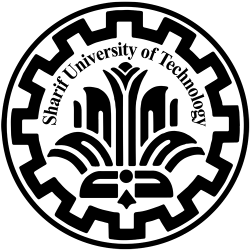
\includegraphics[width=2.3cm]{img/img1.png}}\\
		\vspace{0.3cm}
		
		{\small \bf \emph{Sharif University\\Of\\Technology}}
		
	\end{titlepage}
%
	\setstretch{2}
	\tableofcontents	
	\newpage

% ..................................................................................................
	\setstretch{1.5}
	\section{\LARGE Solutions : }
		\subsection{{\Large Question 1 :} Examples of Markov Chain }
			\begin{enumerate}
				\item{\textbf{Weather model :} 
					
					 The probabilities of weather conditions (modeled as either rainy or sunny), given the weather on the preceding day, , can be represented by a graph .
					 \begin{figure}[htbp]
				 	 \begin{center}
				 	 	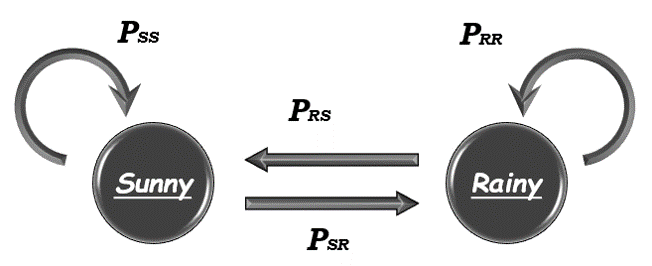
\includegraphics[width= 6cm]{img/weather_Diagram} 
			 	 	 \end{center}
		 	 	 \caption{Weather State diagram}
		 	 	 \end{figure}
		 	 	 }
				 		
				\item{\textbf{Gamblers ruin :}

					Consider a tennis game in Which the the score has reached deuce .
					Suppose that computer wins with the probability P .
					\begin{figure}[htbp]
						\begin{center}
							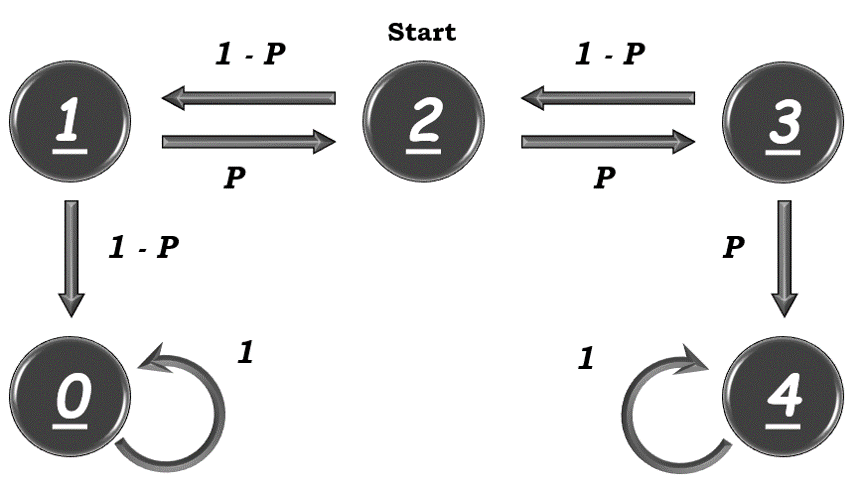
\includegraphics[width= 7cm]{img/tennis_Diagram} 
						\end{center}
						\caption{State diagram}
				\end{figure}
			}
				
				\item{\textbf{Random Walk :}}
				
					A boy walks along a four-block stretch of a Road. If he is at corner 1, 2,
					or 3, then he walks to the left or right with equal probability. He continues until he
					reaches corner 4, which is a Park, or corner 0, which is his home. If he reaches either
					home or the park, he stays there.

					
					The transition matrix is like below : 
					
					\begin{equation*}
					P = 
					\begin{bmatrix}
					1 & 0 & 0 & 0 & 0     \\
					1/2 & 0 & 1/2 & 0 & 0 \\
					0 & 1/2 & 0 & 1/2 & 0 \\
					0 & 0 & 1/2 & 0 & 1/2 \\
					0 & 0 & 0 & 0 & 1
					\end{bmatrix}
					\end{equation*}
				
			\end{enumerate}
			
			
		\vspace{2\baselineskip}
		\subsection{{\Large Question 2}}
			\hspace{\parindent} \large Show that : 
			{$$\displaystyle{\sum_{j=1}^{M} p_{ij} = 1} \hspace{2cm} {\left(\forall\, i \in \chi \right)} $$} 

			\large{\bf \emph{Proof :}}
			\vspace{.8cm}
			
			{$\displaystyle{\sum_{j=1}^{M} p_{ij} = \sum_{j=1}^{M} P[X_{n+1} = j | X_{n} = i]} = \sum_{j=1}^{M} \frac{P[X_{n+1} = j , X_{n} = i]}{P[X_{n} = i]} $}\\
			\vspace{.5cm}
			
			\hspace{1.3cm}{$\displaystyle{= 
							 \frac{\sum_{j=1}^{M} P[X_{n+1} = j , X_{n} = i]}{P[X_{n} = i]} = \frac{P[X_{n} = i]}{P[X_{n} = i]} = 1}$}
				
		\subsection{{\Large Question 3 :} Distribution of Step n }
		\setstretch{2}
		\hspace{\parindent} If in a Markov Sequence {$\left\{X_{n}\right\}_{n=0}^{\infty}$} , 
		distribution of $X_{n}$ is denoted by $\lambda_{n}$ , Prove that :\[\lambda_{n} = \lambda P^n\]

		\large{\bf \emph{Proof 1 :}} By Using Matematical Induction .

		
		N = 0 : \hspace{\parindent} $\lambda_{0} = \lambda$ \hspace{2cm} (Base Case)
		
		Suppose that foe N = k is true , and prove for N = k + 1
		
		N = k : \hspace{\parindent} $\lambda_{k} = \lambda P^k$
		
		and now let's prove for N = k + 1 :
		
		N = k + 1 : \hspace{2\parindent} $\lambda_{k+1} = \lambda P^{k+1} = (\lambda P^k)\cdot P = \lambda_{k}P $
		\bigskip
		
		\setstretch{1.5}
		{It's obviouse that   $\lambda_{k+1} = \lambda_{k}\cdot P$ is true , because it's the Markov
		chain's property
		
		that each step is transformed to the next one, when it's multiplied by P .}
		
		\bigskip
		
		\setstretch{2}
		\large{\bf \emph{Proof 2 :}}
		We know that : \[\lambda_{n} = \lambda_{n-1}\cdot P\]
		
		So we have : \[\lambda_{n} = \lambda_{n-1}\cdot P = (\lambda_{n-2}\cdot P )\cdot P = \cdots = \lambda_{0}\cdot P^n\]
		
		\subsection{{\Large Question 4 :} Higher Order Markov Chain}
		\subsubsection{Markov Chain Of \texorpdfstring{$\bf 2_{nd}$}{Lg} Order}
			If for a sequence $\displaystyle{[X_{n}]_{n=0}^{\infty}}$ we have : \[P[X_{n+1} | X_0 , X_1 , \cdots , X_{n-1} , X_{n}] = P[X_{n+1} | X_{n} , X_{n-1}]\hspace{1cm} \text{(Second Order Markov Chain)}\] Prove that it can be written as a Morkov Chain (First Order Markov Chain) .
			
			\large{\bf \emph{Proof :}} Let's define  $Y_n := (X_n , X_{n+1})$
			
			So Equation : \[P[X_{n+1} | X_0 , X_1 , \cdots , X_{n-1} , X_{n}] = P[X_{n+1} | X_{n} , X_{n-1}]\]
			
	%		\[\bf \Bigg\Downarrow Changes \]
			
			Can be Witten as : \[P[X_{n+1} | X_0 , X_1 , \cdots , X_{n-1} , X_{n}] = P[Y_n| Y_{n-1}]\]
			
			We can show that :
			\[P[Y_n| Y_{n-1}]  = P[ (X_{n+1} , X_n ) | (X_n ,  X_{n-1}) ] = P[X_{n+1} | X_{n} , X_{n-1}]\]
		
		\subsubsection{Markov Chain Of \texorpdfstring{$\bf K_{th}$}{Lg} Order : }
		
		If for a sequence $\displaystyle{[X_{n}]_{n=0}^{\infty}}$ we have : 
		\[P[X_{n+1} | X_0 , X_1 , \cdots , X_{n-1} , X_{n}] = P[X_{n+1} | X_{n} , X_{n-1} , \cdots , X_{n-k}] \]Prove that it can be written as a Morkov Chain (First Order Markov Chain) .
		
		\newpage
		\large{\bf \emph{Proof :}}
		Let's define $Y_{n} := (X_{n-k+1} , X_{n-k+2} , \cdots , X_{n+1})$
		
		So the Equation : \[P[X_{n+1} | X_0 , X_1 , \cdots , X_{n-1} , X_{n}] = P[X_{n+1} | X_{n} , X_{n-1} , \cdots , X_{n-k}] \]
		
		Can be written as :\[P[X_{n+1} | X_0 , X_1 , \cdots , X_{n-1} , X_{n}] = P[Y_n | Y_{n-1}] \]
		
		And we show that : \[P[Y_n | Y_{n-1}] = P[(X_{n+1}, X_n , \cdots , X_{n-k+1}) |(X_{n} , X_{n-1} , \cdots , X_{n-k})]\] \[= P[X_{n+1} | X_{n} , X_{n-1} , \cdots , X_{n-k}]\]
		
		\subsection{\Large Question 5}
		Prove that sequence $[X_{n}]_{n=0}^{\infty}$ , is a Markov Chain with initial distribution of $\lambda$ and transition matrix of $P = [p_{ij}]_{M\times M}$ , If and only if $(\forall\,n$ and $\displaystyle{\{i_N\}_{N=0}^{n} \in\,\chi)}$ we have :\[P[X_0 = i_0 , X_1 = i_1 , \cdots , X_n = i_n] = \lambda_{i_0}p_{i_0i_1}p_{i_1i_2}p_{i_2i_3}\cdots p_{i_{n-1}i_{n}}\]
		
		\large{\bf \emph{Proof :}}
		Suppose we observe a finite realization of the discrete Markov chain and want 
		
		to compute the probability of this random event:
		
		Using Conditional Probability  : \[P[X = x \,, Y= y] = P[X=x | Y=y]\cdot P[Y=y]\]
		We have :
		\[P[X_n = i_n , X_{n-1} = i_{n-1} , \cdots , X_1 = i_1 , X_0 = i_0]\]\[= P[X_n = i_n | X_{n-1} = i_{n-1} , \cdots , X_1 = i_1 , X_0 = i_0]\cdot P[X_{n-1} = i_{n-1}, \cdots , X_1 = i_1 , X_0 = i_0]\]
		\[ = p_{i_{n-1}i_{n}} \cdot P[X_{n-1} = i_{n-1} | X_{n-2} = i_{n-2} , \cdots , X_1 = i_1 , X_0 = i_0]\cdot P[X_{n-2} = i_{n-2}, \cdots , X_1 = i_1 , X_0 = i_0]\]
		\[=\, \, \vdots\]
		\[= p_{i_{n-1}i_{n}}p_{i_{n-2}i_{n-1}} \cdots p_{i_0i_1} P[X_0 = i_0]\]
		\[= \lambda_{i_0}\cdot p_{i_{0}i_{1}}\cdot p_{i_{1}i_{2}}\cdots p_{i_{n-2}i_{n-1}}\cdot p_{i_{n-1}i_{n}} \]
		
		\subsection{\Large Question 6}
		Draw the state diagram for the below transition matrix :
		
		
			\begin{equation*}
			P = 
				\begin{bmatrix}
					0 & 1 &0\\
					0 & \frac{2}{3} &\frac{1}{3} \\
					\frac{1}{2} & \frac{1}{2} & 0\\
				\end{bmatrix}
			\end{equation*}
			
			Here is the State Diagram :
			
			\begin{figure}[htbp]
				\begin{center}
					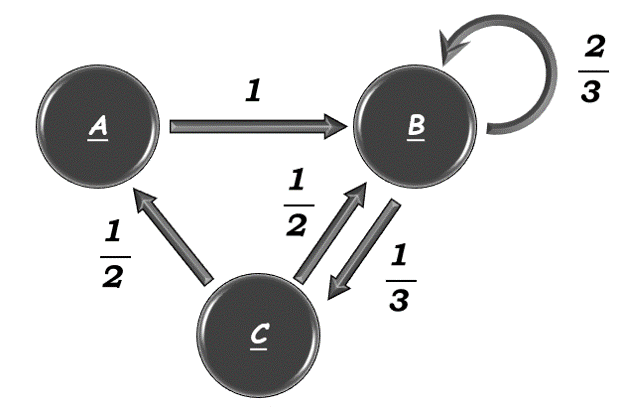
\includegraphics[width= 6cm]{img/q6} 
				\end{center}
				\caption{State diagram of matrix P}
			\end{figure}
		\newpage
		
		\subsection{{\Large Question 7 :} The Chapman–Kolmogorov equations}
		
		First , Let's mention a proposition that ,
		In general, we define the n-stage transition probabilities, denoted as $P^{(n)}_{ij}$, by 
		\[p_{ij}(m , m+n) = P[X_{m+n} =j , X_{m} = i] = p^{(n)}_{ij}\]
		For a Markov chain, $P_{ij}$ represents the probability that a system in state i
		will enter state j at the \textbf{next transition}. We can also define the \textbf{n-stage transition}
		probability $P^{(n)}_{ij}$ that a system presently in state i will be in state j after n additional
		transitions.
		
		\noindent{Let's Start by the proof for the Equation }\[P[X_{m+n} =j , X_{m} = i] = P[X_{n} =j , X_{0} = i]  = p^{(n)}_{ij}\]
		\setstretch{2.5}
		\noindent{\large {\bf{Proposition 7.1 :}}}
		
		\noindent{\large{\bf \emph{Proof :}}}
		
		$P[X_{m+n} =j | X_{m} = i] =$
		
		$= \displaystyle{\sum_{i_{m+1}, i_{m+2} , \cdots , i_{m+n-1}} P[X_{m+n}=j|X_{m+n-1} = i_{m+n-1}]\times\cdots\times P[X_{m+1} = i_{m+1} | X_{m} = i_m]}$
		
		$= \displaystyle{\sum_{i_{m+1}, i_{m+2} , \cdots , i_{m+n-1}} P[X_{n}=j|X_{n-1} = i_{m+n-1}]\times\cdots\times P[X_{1} = i_{m+1} | X_{0} = i_m]}$
		\bigskip
		
		$= P[X_n = j | X_0 = i] = p^{(n)}_{ij}$
		\setstretch{2}
		
		\noindent{Now , Let's use the \textbf{Proposition 7.1} to prove that :}
		
		 \[p^{(n+r)}_{ij} = p_{ij}(m , m+n+r) = \sum_{k} p_{ik}(m , m+n)\cdot p_{kj}(m+n , m+n+r)\]
		
		\newpage
		\setstretch{3}
		\large{\bf \emph{Proof :}}

		$\displaystyle{p^{(n+r)}_{ij} = P[X_{n+r}=j | X_0 = i] = \sum_{k \in S} P[X_{n+r}=j, X_{n}=k | X_0 = i]}$
		
		$\displaystyle{ \hspace{1.1cm}=\sum_{k \in S} P[X_{n+r}=j | X_{n}=k , X_0 = i]= \sum_{k \in S} P[X_{n+r}=j | X_{n}=k]\cdot P[X_{n}=k | X_{0}=i] } $
		
		$\displaystyle{ \hspace{1.1cm}= \sum_{k \in S} p^{(n)}_{ik}\cdot p^{(r)}_{kj} = \sum_{k \in S} p_{ik}(m,m+n) \cdot p_{kj}(m+n,m+n+r) }$
		
		\noindent{Now if we know that $ \rightarrow P(m , m+n) = [p_{ij}(m , m+n)]_{M\times M}$}
		
		\setstretch{2}
		\noindent{Prove that $\Rightarrow P(m , m+n) = P^n$ \hspace{1cm} ($\ast$)}
		
		\large{\bf \emph{Proof :}}
		
		\textbf{First}, We know that the $i_{th}$ row and $j_{th}$ column of matrix $P^{n}$ is denoted by $p^{(n)}_{ij}$. 
		
		\textbf{Second}, We know that each member of matrix $P(m,m+n)$ is denoted by $p_{ij}(m,m+n)$. 
		
		For the proof , let's show that both matrices are the same in the $i_{th}$ row and $j_{th}$ column .
		
		So we have :
		 
		\setstretch{3}
		
		$p_{ij}(m,m+n) = P[X_{m+n} =j | X_{m} = i] =$
		
		$= \displaystyle{\sum_{i_{m+1}, i_{m+2} , \cdots , i_{m+n-1}} P[X_{m+n}=j|X_{m+n-1} = i_{m+n-1}]\times\cdots\times P[X_{m+1} = i_{m+1} | X_{m} = i_m]}$
		
		$= \displaystyle{\sum_{i_{m+1}, i_{m+2} , \cdots , i_{m+n-1}} P[X_{n}=j|X_{n-1} = i_{m+n-1}]\times\cdots\times P[X_{1} = i_{m+1} | X_{0} = i_m]}$
		\bigskip
		
		$= P[X_n = j | X_0 = i] = p^{(n)}_{ij}$
		
		Then since : $ p_{ij}(m,m+n) = p^{(n)}_{ij} \Longrightarrow  P(m , m+n) = P^n$
		
		\newpage
		\setstretch{2}
		
		\subsection{{\Large Question 8 :} Classifiction of States}
		
		$\bullet$ Accessible: State j is accessible from state i if $P^{(n)}_{ij} > 0 \hspace{1cm} (\forall n \geq 0)$\[P^{(n)}_{ij} > 0 \hspace{1cm} (\forall n \geq 0) \hspace{0.6cm}\Longleftrightarrow \hspace{0.6cm} i\rightarrow j\]
		Now we see that $ (i\rightarrow j)$ is equivalent to : $P[\text{ ever enter } j\,| \text{ start in } i ] > 0 $
		
		\setstretch{1.5}
		\noindent{\large {\bf{Proposition 8.1 :}}}
		\[P[\text{ ever enter } j\,| \text{ start in } i ]\]	
		 \[= P[\cup_{n=0}^{\infty}\{X_n = j\} | X_0 = i]\]
		\[ \leq \sum_{n=0}^{\infty} P[X_n =j | X_0 = i]\]\[= \sum_{n=0}^{\infty} p^{(n)}_{ij}\]
		
		\setstretch{2}
		
		\noindent{Hence if $p^{(n)}_{ij} = 0$ (for all n) , $P[\text{ ever enter } j\,| \text{ start in } i ] = 0$ . }
		
		\noindent{On the other hand,}
		
		\noindent{\large {\bf{Proposition 8.2 :}}}
		\[P[\text{ ever enter } j\,| \text{ start in } i ]\]	
		\[= P[\cup_{n=0}^{\infty}\{X_n = j\} | X_0 = i]\]\[ \hspace{4cm} \geq P[X_n =j | X_0 = i] \hspace*{3cm} \text{(for any n)}\]\[= p^{(n)}_{ij}\]
		\noindent{If $p^{(n)}_{ij} > 0$ for some n, $P[\text{ ever enter } j\,| \text{ start in } i ] \geq p^{(n)}_{ij} > 0 $ .}
			
		\newpage
	
		\subsection{{\Large Question 9}}
			First , Let's define \textbf{Equivalance relation}\\*
			$ \bullet $ An equivalence relation ``$ \sim $'' is a binary relation between elements of a set satisfying
			
			1. Reflexivity: $ i \sim j$ for all $i$
			
			2. Symmetry: $ i \sim j \Longrightarrow j \sim i$ 
			
			3. Transitivity: $ i \sim j , j \sim k \Longrightarrow i \sim k$
			
			\noindent{\large {\bf{Proposition 9.1 :}} Communication of states is an equivalence relation.}
			
			\large{\bf \emph{Proof :}} Reflexivity and symmetry are clear. To prove transitivity,
			let $i \leftrightarrow j$ and $j \leftrightarrow k$.
			
			We then want to show that $i \leftrightarrow k$ .
			
			$\bullet$ Note that $i \rightarrow j$ if and only if the transition diagram contains a path from $i$ to $j$.
			
			So there is a path from $i$ to $j$ and from j to k. Concatenate the two to obtain a 
			
			path from $i$ to $k$, which testifies to the fact that $i \rightarrow k$ .
			\bigskip
			
			Analogously, we have $k \rightarrow i$ and conclude that $i \leftrightarrow k$ .
		
		\subsection{{\Large Question 10}}
		
		Find the communication classes of a markov chain with this transition matrix :	
			\begin{equation*}
				P = 
				\begin{bmatrix}
					\frac{1}{2} &0&0&0&\frac{1}{2}\\
					0&\frac{1}{2}&0&\frac{1}{2}&0\\
					0&0&1&0&0\\
					0&\frac{1}{4}&\frac{1}{4}&\frac{1}{4}&\frac{1}{4}\\
					\frac{1}{2} &0&0&0&\frac{1}{2}\\
					
				\end{bmatrix}
			\end{equation*}
			Which classes are close ?
			
			\newpage
			\noindent{Let's draw the state diagram of the matrix : }
			
			\begin{figure}[htbp]
				\begin{center}
					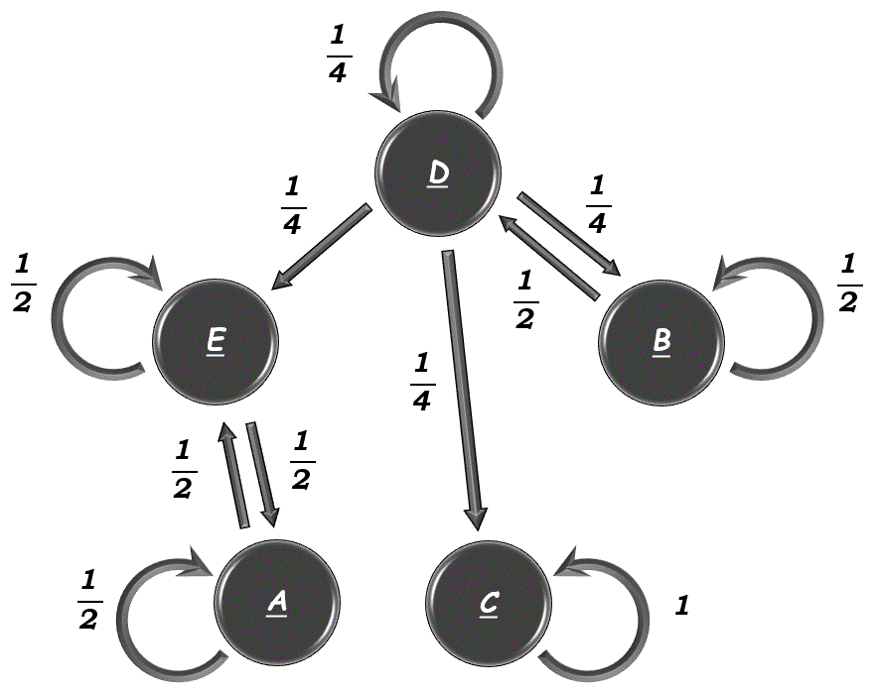
\includegraphics[width= 6cm]{img/q10} 
				\end{center}
				\caption{State diagram}
			\end{figure}
		
		\noindent {The communication classes are : \{A\} , \{B\}, \{C\}, \{D\}, \{E\} , \{A,E\} , \{B,D\}}\\*
		The close communication classes are : \{C\}, \{A,E\}
	
	\subsection{{\Large Question 11 :} Random walk (one dimentional)}
		There's a man walking on a line of integer numbers, steps forward with probability of $p$ and steps back with $1-p$ , and now we're gonna find the period of the states .(The start point is at $X_0 = 0$).
		
		\noindent{The mathematically modeled form of the problem is :}\[P[x_{n+1} = i+1 | X_n = i] = p \text{\hspace{.6cm} and \hspace{.6cm}} P[x_{n-1} = i-1 | X_n = i] = p\]
		
		\noindent{The states of this markov chain are integer numbers. So, we will have \textbf{odd} or \textbf{even} periods.} 
		$\bullet$ Define $p^{(n)}_{ii}$ is the probability of starting at state $i$ and turn back to state $i$ after $n$ steps .
		
		\noindent{It's \textbf{obvious} that if you are in the state {\boldmath$i$}, it's impossible to reach state {\boldmath$i$} again after an odd number of steps . }
		
		E.g, suppose that the man is on the state \emph{0} , it's obvious that there's noway he can
		
		turn back to the \emph{0} state by moving odd (1,3,5,$\cdots$) steps; So, we have :
		
		\begin{center}
			$p^{(n)}_{ii} = 0 \hspace{0.7cm} ,\,\, (\forall \,\, {\boldsymbol{n}} = 2k+1 \,\,;\,\, {\boldsymbol{k}} = 0, 1, 2, \cdots)$
		\end{center}
	
	We want to show that for all {\boldmath$i$} states on the line , \[p^{(n)}_{ii} > 0 \hspace{.8cm}, \,\,\, (\forall \,\, {\boldsymbol{n}} = 2k \,\,;\,\, {\boldsymbol{k}} = 0, 1, 2, \cdots)\]
	As we know that moves with even steps can be modeled by 2-step moves, Let's Prove that :
	\[p^{(2)}_{ii} > 0 \hspace{.8cm}, \,\,\, ({\boldsymbol{n}} = 2)\]
	
	\noindent{\large{\bf \emph{Proof :}}}
	
		\[p^{(2)}_{ii} = P[X_2=i | X_0 = i] = \sum_{k}P[X_2=i, X_1 = k | X_0 = i] \]
		\[= \sum_{k}P[X_2=i | X_1 = k , X_0 = i]\cdot P[X_1 =k | X_0 = i]\]
		\[= \sum_{k}P[X_2=i | X_1 = k]\cdot P[X_1 =k | X_0 = i]\]
		\[= P[X_2=i | X_1 = i-1]\cdot P[X_1 =i-1 | X_0 = i] + P[X_2=i | X_1 = i+1]\cdot P[X_1 =i+1 | X_0 = i]\]
		\[= p(1-p) + (1-p)p = 2p(1-p) > 0\]
	So we have : \hspace{1cm} $( d_i = \gcd \{{\boldsymbol{n}} = 2k \geq 1 ; {\boldsymbol{k}} = 1, 2, \cdots\} = 2)$ \hspace{0.6cm} (even steps)
	
	\subsection{{\Large Question 12}}
		\emph{Period} is a communication class property. Namely, $i \leftrightarrow j \Longrightarrow d_i = d_j$
		
		\noindent{Let $p^{(k)}_{ij}$ denote the k-step transition probability from state $i$ to $j$ and let $d_i$ denote $i$'s period. Suppose that i and j communicating and $\alpha = p^{(k)}_{ij} > 0$ and $\beta = p^{(l)}_{ji}$ for some $k$ and $l$. Then by Chapman-Kolmogrov equations :\[p^{(k+l)}_{ii} = \sum_{k} p^{(k)}_{ik}p^{(l)}_{ki} \,\,\,\, \geq \,\,\,\, p^{(k)}_{ij}p^{(l)}_{ji} = \alpha \beta  > 0\]  
		So , $(k+l)$ is multiple of $d_i \Longrightarrow d_i | (k+l)$ 
			
		\noindent{Suppose now that $m \in \{ n\,\,\, ;\,\,\, p^{(n)}_{jj} > 0\}$ then again using Chapman-Kolmogrov equations we have that $p^{(k+l+m)}_{ii} > 0$ (you go from $i$ to $j$, go off somewhere and return to $j$, and then return to $i$), so $d_i | (k+l+m)$ and so we get that $d_i | m$ . Since $d_i | m $ and $d_i | (k+l+m)$ , so $d_j \geq d_i$.
		Now exchanging the roles of i and j we get that $d_i \geq d_j$ . 
		
		\noindent{So we conclude that $d_i = d_j$} .
		
		\subsection{{\Large Question 13 :} Hitting probabilities }
		
			Let's prove that the vector of hitting probabilities, $h^A = [h^{A}_1 , h^{A}_2, \cdots , h^{A}_M]$ , minimal answer of the following system of linear equations:
			\begin{equation}
			h^{A}_i = 
				\begin{cases}
					1 \hspace{3cm} & \forall i \in A \\
					\sum_{j \in \chi} p_{ij} h^{A}_{j} \hspace{2cm} & \forall i \notin A
				\end{cases}
			\end{equation}
			
		\noindent{\large{\bf \emph{Proof :}}}
		We consider to cases seperately . If $X = i \in A $ , then $H^{A} = 0$ and $h^{A}_i = 1$ .
		
		\noindent{On the other hand, if $X = i \notin A$, then $H^{A} \geq 1$, so by the Markov property :}\[P_i[H^{A} < \infty | X_1 = j] = P[H^{A} < \infty] = h^{A}_j\]
		Now, Total probability theorem implies that :\[h^{A}_i  = P_i[H^{A} < \infty] = \sum_{j\in S}P_i[H^{A} < \infty | X_1 = j]P_i[X_1=j] = \sum_{j\in S} p_{ij}h^{A}_j\]
		
		\newpage
		
		\subsection{{\Large Question 14}}
	
		Let's prove that the vector of mean hitting times, $k^{A}$ ,is the minimal non-negative solution to the following system of linear equations :
		\begin{equation}
		k^{A}_i = 
			\begin{cases}
			0 \hspace{3cm} & \forall i \in A \\
			1+\sum_{j \in \chi} p_{ij} k^{A}_{j} \hspace{2cm} & \forall i \notin A
			\end{cases}
		\end{equation}
		
		\noindent{\large{\bf \emph{Proof :}}}
		We consider to cases seperately . If $X = i \in A $ , then $H^{A} = 0$ and $k^{A}_i = 0$ .
		
		\noindent{On the other hand, if $X = i \notin A$, then $H^{A} \geq 1$, so by the Markov property :}\[E_i[H^{A}| X_1 = j] = 1 + E_j[H^{A}]\]consequently, by the partition theorem for the expectations,
		\[k^{A}_i = E_i[H^{A}] = \sum_{j \in S} E_i[H^{A} | X_1 = j ]P_i[X_1 = j] = \sum_{j \in S} p_{ij}k^{A}_j\]
		
		\subsection{{\Large Question 15 :} Example}
		According to the transition matrix : 
%		\begin{equation*}
%		P = 
%			\begin{bmatrix}
%				1&0&0&0\\
%				\frac{1}{2}&0&\frac{1}{2}&0\\
%				0&\frac{1}{2}&0&\frac{1}{2}\\
%				0&0&0&1
%			\end{bmatrix}
%		\end{equation*}

	\noindent{{\large\textbf{1. Solution : }}Put $h_i = P_i[H^{\{4\}} < \infty]$. Clearly $h_1 = 0$ and $h_4 = 1$ and by using markov property we have :}
	\begin{center}
		$h_2 = \frac{1}{2} (h_1 + h_3) \hspace{1.5cm} h_3 = \frac{1}{2} (h_2 + h_4)$
	\end{center}
	As the result : $h_2 = \frac{1}{2} h_3 = \frac{1}{2} (\frac{1}{2}h_2 + \frac{1}{2})$ , that is $h_2 = \frac{1}{3}$ and $h_3 = \frac{2}{3}$ .
	
	\noindent{{\large\textbf{2. Solution : }} Put $k_i = E_i[h^{\{1,4\}}]$. Clearly, $k_1 = k_2 = 0$ and by using Markov chain property we have :  $\hspace{.5cm}k_2 = 1 + \frac{1}{2} (k_1 + k_3) \hspace{1.5cm} k_3 = 1 + \frac{1}{2} (k_2 + k_4)$}
	
	\noindent{As the result : $k_2 = 1+ \frac{1}{2}k_3 = 1+ \frac{1}{2} (\frac{1}{2}k_2)$ }, that is $k_2 = k_3 = 2$ .
	
	{\tiny \textcolor{white}{\subsection{16}}}
	\newpage
	\subsection{{\Large Question 17 :}}
	
		Let's More generally prove that :
		\begin{center}
			State ${\mathbf i}$ is \textbf{recurrent} $ \,\,\,\Longleftrightarrow \,\,\, \sum_{n=1}^{\infty} p^{(n)}_{ii} = \infty$
			
			State ${\mathbf i}$ is \textbf{transient} $ \,\,\,\Longleftrightarrow \,\,\, \sum_{n=1}^{\infty} p^{(n)}_{ii} < \infty$
		\end{center}
	
	\noindent{\large{\bf \emph{Proof :}}}
	First, Let's remind some defenitions :
	
	Definition 17.1 : A state $i \in S$ is recurrent if : 
		\[P[\,\exists\,\, n \geq 1 : X_n=i | X_0 =i] = 1\]
		
	Definition 17.2 : A state $i \in S$ is recurrent if : 
	\[P[\,\exists\,\, n \geq 1 : X_n=i | X_0 =i] = 0\]
	
	Definition 17.2 : A state $i \in S$, Denote $f_{ii}$, the probability that a Markov chain which 
	
	starts at $i$ returns to $i$ at least once, that is :
	\[f_i = P[\,\exists\,\, n \in {\mathbb N}  : X_n = i ]\]
	
	Then , 
	
	1. State $i$ is recurrent if and only if  $f_i = 1$
	
	2. State $i$ is transient if and only if  $f_i < 1$
	
	Now let's have the main question :
	
	Let the Markov chain start at state $i$. Consider the random variable\[V_i := \sum_{n=1}^{\infty} I{\{X_n = i\}}\]
	\newpage
	
	Which counts the number of returns of the Markov chain to state $i$. Note that the random
	
	variable $V_i$ can take the value $+\infty$ . Then, \[P[B_k] = P[V_i \geq k] = f^k_{i} \hspace{1cm} (\forall\,\, k \in {\mathbb N} ) \]
	Thus, the expectation of $V_i$ can be computed as follows:
	\[\hspace{-6cm}(17.1) \hspace{2.5cm} {\mathbb E}_i[V_i]  = \sum_{k=1}^{\infty} P_i[V_i \geq k] = \sum_{k=1}^{\infty} f^{k}_i \]
	On the other hand ,
	\[\hspace{-1.5cm}(17.2) \hspace{2cm} {\mathbb E}_i[V_i]  = {\mathbb E}_i\Bigg[\sum_{n=1}^{\infty} I{\{X_n = i\}}\Bigg] = \sum_{n=1}^{\infty} {\mathbb E}_i[I{\{X_n = i\}}] = \sum_{n=1}^{\infty} p^{(n)}_{ii}\]
	
	\noindent{\textbf{Case 1 :}  Assume that state i is recurrent. Then, By definition 17.3  $\Rightarrow f_i = 1$ . }
	
	\noindent{It follows by 17.1 that, ${\mathbb E}_i[V_i] = \infty$ .\\*
	(In fact, $P_i[V_i = +\infty] = 1$ since $P[v_i \geq k] =1$ for every $k \in {\mathbb N}$) . \\*Hence, by 17.2,  $\sum_{n=1}^{\infty} p^{(n)}_{ii} = \infty$}

	\noindent{\textbf{Case 2 :} Assume that state i is transient. Then, By definition 17.3  ,$f_i < 1$.Thus, By 17.1, ${\mathbb E}_i[V_i] < \infty$. Hence, By 17.2, $\sum_{n=1}^{\infty} p^{(n)}_{ii} < \infty$ . }
	
	\vspace{-3cm}{\tiny \textcolor{white}{\subsection{18}}}
	\vspace{0.5cm}
	{\tiny \textcolor{white}{\subsection{19}}}
	
	\subsection{{\Large Question 20 :} Recurrence and transience of random walks}
	A simple random walk on ${\mathbb Z}$ is a Markov chain with state space ${S = \mathbb Z}$ andtransition probabilities : \[p_{i,i+1} = p\hspace{1cm} , \hspace{1cm} p_{i,i-1} = 1-p\hspace{1cm} i \in {\mathbb Z}\]
	
	\newpage
%	rand_walk
	\noindent{So, from every state the random walk goes one step to the forward with probability $p$, or one step back with probability $1-p$; \\* Look at Figure 5 that simulates \textbf{Random walk} for 200 steps on ${\mathbb Z}$ with $p = \frac{1}{2}$ . }
	
	\begin{figure}[htbp]
		\begin{center}
			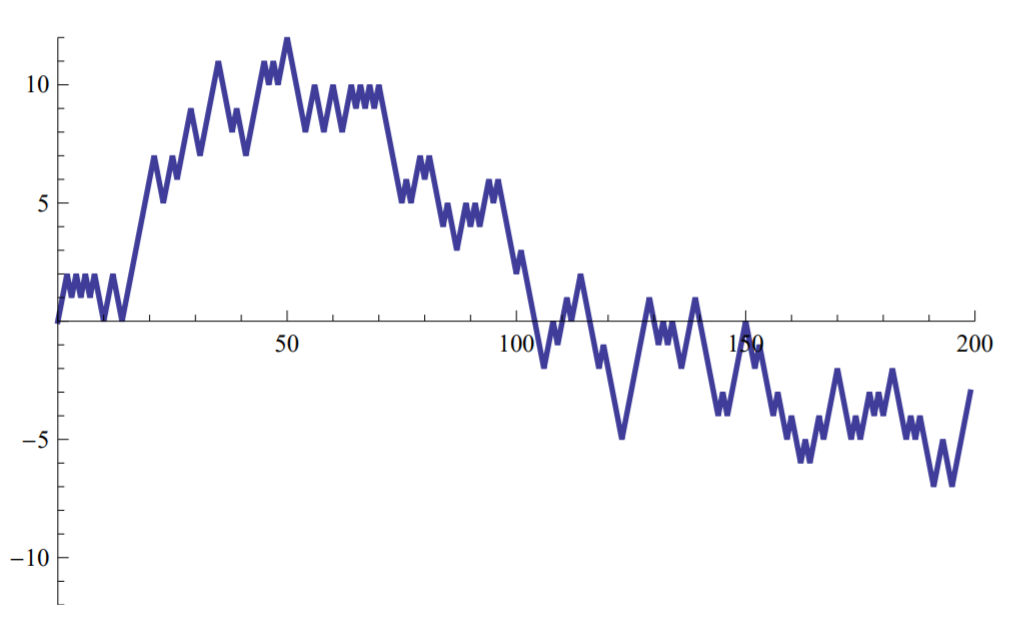
\includegraphics[width= 6cm]{img/rand_walk} 
		\end{center}
		\caption{Random Walk Simulation with $p = \frac{1}{2}$}
	\end{figure}

	\noindent{\textbf{Theorem 20.1 :} If $p=\frac{1}{2}$, then any state of the simple random walk is recurrent. \\* If $p \neq \frac{1}{2}$ then any state is transient.}
	
	\textcolor{white}{\section{\LARGE References :}}}
	\newpage
	
	
		\noindent{\Huge \bf References : }
		\vspace{1cm}
		
		\noindent{\Large \textbf{\LARGE1} . Probability - Random Variables and Stochastic Processes.\\* (by:Athanasios Papoulis)}
		\bigskip
		
		\noindent{\Large \textbf{\LARGE2} . A First Course in Probability (9th Edition). (by: Sheldon Ross)}
		
		\noindent{\Large \textbf{\LARGE3} . Cambridge University Statistics Courses :\\* ( \href{https://www.training.cam.ac.uk/course/ucs-stats\_diy}{https://www.training.cam.ac.uk/course/ucs-stats\_diy} )}
		
		\noindent{\Large \textbf{\LARGE4} . Discrete Probability Models and Methods: Probability on Graphs and Trees, Markov Chains and Random Fields, Entropy and Coding .\\* ( by : Pierre Brémaud ) .}
		
		
		

	
\end{document}